%%%%%%%%%%%%%%%%%%%%%%%%%%%%%%%%%%%%%%%%%%%%%%%%%%%%%%%%%%%%%%%%%%%%%%%%%%%
%% This file is part of the book
%%
%% Algorithmic Graph Theory
%% http://code.google.com/p/graph-theory-algorithms-book/
%%
%% Copyright (C) 2009, 2010, 2011 Minh Van Nguyen <nguyenminh2@gmail.com>
%%
%% See the file COPYING for copying conditions.
%%%%%%%%%%%%%%%%%%%%%%%%%%%%%%%%%%%%%%%%%%%%%%%%%%%%%%%%%%%%%%%%%%%%%%%%%%%

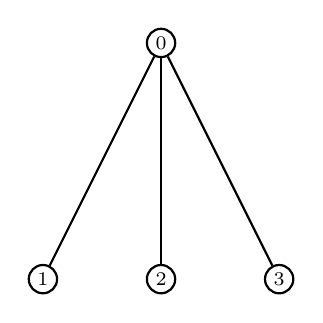
\begin{tikzpicture}
[nodeDecorate/.style={shape=circle,inner sep=1.5pt,draw,thick},%
  lineDecorate/.style={-,thick},%
  scale=1.5]
\scriptsize
%% nodes or vertices
\foreach \nodename/\x/\y in {1/0/0, 2/1/0, 3/2/0, 0/1/2}
{
  \node (\nodename) at (\x,\y) [nodeDecorate] {$\nodename$};
}
%% edges or lines
\path
\foreach \startnode/\endnode in {0/1, 0/2, 0/3} {
  (\startnode) edge[lineDecorate] node {} (\endnode)
};
\end{tikzpicture}
